%%%%%%%%%%%%%%%%%%%%%%%%%%%%%
%Since : 2019/04/03
%Update: 2019/04/08
% -*- coding: utf-8 -*-
%%%%%%%%%%%%%%%%%%%%%%%%%%%%%

\chapter{Excelによる統計処理1}

\section{目的}

Excelの操作を通し,データ処理の基礎とグラフの作成の仕方を学ぶ.

\section{理論}

\subsection{統計とは}

統計や確率は様々な場面で用いられています.
それはなぜでしょうか.
一つの目的は,全体の特徴もしくは規則性を捉えるために用いられます.
皆さんは,大学受験で大学の偏差値や合格者のセンター試験の平均点などを調べたのではないでしょうか.
偏差値やセンター試験の平均点は統計の結果得られた立派な量です.
これらの数値は,大学の合格者の手段の特性を表しています.
今後,卒業研究はもちろん就職してからも大量のデータを扱い,集団の特性や規則性を調べることになると思います.
この演習を通じ,統計の基礎とExcelによる簡単な統計処理を身につけてください.

\subsection{データ}

$N$個のデータがあるとするとそのデータのセット$X$は次のように表されます.
\begin{equation}
    \label{eq:2}
    X = \{x_1, x_2, ..., x_N\}
\end{equation}

\subsection{代表値}

例えば,表\ref{tab:sample}に示すデータセットがあったとします.
このデータの特徴は何でしょうか.
といきなり言われても困りますよね.
データセットの特徴を1つの値で表したいときに用いるのが代表値です.
今回用いる代表値は,平均,中央値,分散,標準偏差です.

\begin{table}[tb]
    \caption{データ}
    \centering
    \begin{tabular}{cccccccccc}
       82 & 66 & 39 & 66 & 54 & 56 & 58 & 72 & 53 & 60 \\
       69 & 79 & 71 & 68 & 50 & 68 & 61 & 66 & 74 & 77 \\
       74 & 72 & 73 & 56 & 47 & 59 & 56 & 76 & 69 & 67 \\
       87 & 66 & 57 & 45 & 84 & 53 & 47 & 52 & 49 & 74 \\
       83 & 69 & 87 & 61 & 59 & 64 & 66 & 69 & 79 & 68 \\
       55 & 68 & 50 & 66 & 60 & 69 & 60 & 58 & 83 & 72 \\
       74 & 79 & 65 & 77 & 52 & 65 & 48 & 56 & 76 & 65 \\
       63 & 62 & 63 & 77 & 72 & 68 & 69 & 59 & 63 & 82 \\
       63 & 68 & 80 & 61 & 48 & 58 & 55 & 61 & 54 & 66 \\
       69 & 56 & 79 & 61 & 62 & 61 & 65 & 65 & 75 & 69 \\
    \end{tabular}
    \label{tab:sample}
\end{table}

\paragraph{平均}
平均$\mu$は集団の値の重心を表す最も頻繁に用いられる代表値です.
平均は次の式で表されます.
\begin{equation}
    \mu = \frac{1}{N} \sum_{i=1}^{N} x_i
\end{equation}
皆さんおなじみの平均です.表\ref{tab:sample}のデータの平均は65.09です.


\paragraph{中央値}
中央値はデータを大きさ順で並べ替えて,順番としてちょうど真ん中にあたる値のことです.
例えば,$\{1, 4, 5, 7, 8\}$のようなデータがあったとすると,中央値は順番的に真ん中の5となります.
例のデータの数は奇数でしたので,順番としての中央を決定できましたが,データの数が偶数の場合はどうしたら良いでしょうか.
例えば,$\{1,3,4,5,7,9\}$のようなデータがあったとすると,ちょうど真ん中の値はありません.このような場合は,真ん中の2つの値,4と5を足して2で割った値,すなわち4.5が中央値となります.
表\ref{tab:sample}のデータの中央値は65.5です.
中央値は,平均に対して利点があります.後のほど行う演習で確かめましょう.

\paragraph{分散と標準偏差}
分散はデータのばらつき具合を表します.
分散は次の式で表されます.
\begin{equation}
    \sigma^2 = \frac{1}{N} \sum_{i=1}^{N} (x_i - \mu)^2
\end{equation}
分散の平方根を標準偏差といいます.
表\ref{tab:sample}のデータの分散は約102で標準偏差は約10.1です.

\subsection{度数分布表とヒストグラム}

生データを並べただけでは,それが持つ特徴を直感的に理解することは難しいです.
そこで,データの整理の方法の一つに,度数分布表があります.
度数分布表は,データの取りうる範囲をいくつかの階級に分け,それぞれ階級にあるデータの数(度数)を表したものです.
表\ref{tab:hist}に度数分布表の例を示します.


この度数分布表を図で表したものがヒストグラム(図\ref{fig:histogram})です.
ヒストグラムの横軸は階級を表し,縦軸が度数を表します.
つまり,棒の長さ(面積)が階級に占めるデータの多さを表すことになります.
ヒストグラムに形状を分布といいます.
分布の形状はデータの特徴として非常に重要です.



\begin{figure}[tb]
    \begin{minipage}{0.5\hsize}
    \centering
    \caption{度数分布表}
    \begin{tabular}{c|c}
     階級          & 度数 \\ \hline
     0以上9以下   & 0 \\
     10以上19以下  & 0 \\
     20以上29以下  & 0 \\
     30以上39以下  & 1 \\
     40以上49未満  & 6 \\
     50以上59未満  & 22\\
     60以上69未満  & 43\\
     70以上79未満  & 20\\
     80以上89未満  & 8 \\
     90以上99未満  & 0 \\
     100以上       & 0 \\
     合計          & 100
    \end{tabular}
    \label{tab:hist}
    \end{minipage}
    \begin{minipage}{0.5\hsize}
    \centering
    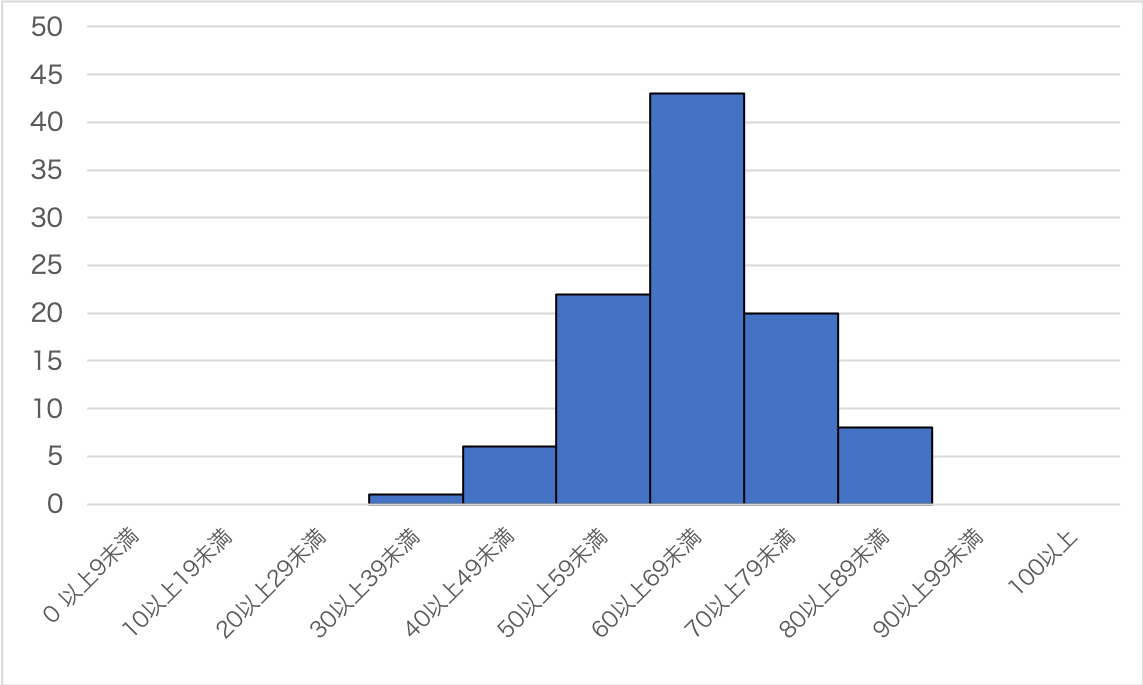
\includegraphics[width=6cm]{chap1/hist.png}
    \makeatletter
    \def\@captype{figure}
    \makeatother
    \caption{ヒストグラム}
  \label{fig:histogram}
\end{minipage}
\end{figure}

\clearpage

\section{Excel実験}

\subsection{データ形式}

データを保存するためのデータ形式は様々ありますが,この演習ではcsvファイルとxslxファイルを用います.
csvファイルは,Comma-Separated Valesファイルの略です.
その名の通り,csvファイルの中身は,データがカンマで区切ってあるだけのテキストファイルです.
単なるテキストファイルですので,どのようなコンピュータを使っている人でも必ず見ることができます.
csvファイルはExcelなど表計算ソフトが入っていれば,表計算ソフトに関連付けされています.
ただし,csvファイルはあくまでも単なるテキストファイルですので,表計算ソフトによる関数による自動計算,作成したグラフ,文字の装飾,表の罫線などは保存されません.
xslxファイルはExcel2007以降で標準的に用いられるファイルです.データだけではなく,関数による自動計算,作成したグラフ,文字の装飾,表の罫線なども保存されます.
この演習では,データはcsvファイルで提供しますが,演習結果の保存はxslxファイルにしましょう.

\subsection{総和,平均,中央値,分散}

Excelでの総和の計算は次の手順で行います.

\begin{enumerate}
    \item 総和を入力したいセルを選択する.
    \item ``=sum(''と入力する.
    \item 総和を計算したいセルをマウスで選択する.
    そうすると``(''の後ろにセル番号が入力される(図\ref{fig:sum}).
    また,データのセル番号を直接入力することで,マウスで選択する操作と同様のことができます.
    例の場合では,セルA1からA5までの総和なので``=sum(A1:A5)''と書きます.
    \footnote{データを選択する方法はいくつかあります.
      皆さんの慣れた方法でやってください.
      また,Excelも自動でいろいろやってくれるので,閉じカッコが保管される場合もあります.
      臨機応変に対応してください.}
    \item ``)''を入力する.
\end{enumerate}

同じやり方で,平均,分散,標準偏差が計算できます.
平均なら``SUM''の部分を``MEAN''に変えます.代表値とexcelの関数の関係を表\ref{tab:funcs}に示します
\footnote{分散や標準偏差に関連する関数は複数あります.
  それぞれ意味が違います.
  その意味はこの講義で扱う範疇を超えているので説明しません.
  興味がある人は調べてみましょう.}.

\begin{figure}[htbp]
    \begin{minipage}{0.5\hsize}
        \centering
        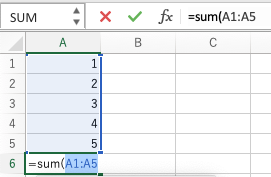
\includegraphics[width=6cm]{chap1/sum.png}
        \caption{総和を計算したいセルを選択した状態.}
        \label{fig:sum}
    \end{minipage}
    \begin{minipage}{0.5\hsize}
        \centering
        \makeatletter
        \def\@captype{table}
        \makeatother
        \caption{代表値とExcelの関数}
        \begin{tabular}{|c|c|}
          \hline
          総和     & SUM\\ \hline
          平均     & MEAN\\ \hline
          分散     & VAR.P\\ \hline
          標準偏差 & STDEV.P \\ \hline
          最大値   & MAX \\ \hline
          最小値   & MIN \\ \hline
        \end{tabular}
        \label{tab:funcs}
    \end{minipage}
\end{figure}

\paragraph{演習}
アヤメデータiris.csv内にあるがく片の長さ,がく片の幅,花びらの長さ,花びらの幅についてそれぞれ平均,中央値,分散,標準偏差を求めなさい.

\paragraph{演習}
gaussian.csvに書かれている数値の平均と中央値を求めなさい.そして,平均値と中央値の差について考察しなさい.ただし,gaussian.csvは,表\ref{tab:sample}の最後のデータを500に置き換えたものです.

\subsection{度数分布表}
\label{sec:freq}

Excelを用い,データ (表\ref{tab:sample})から図\ref{fig:freq}のような度数分布表を作るためには次の手順が必要です.

\begin{enumerate}
    \item まず,図\ref{fig:before_freq}のA列のようにExcelにデータを入力します.
    \item 次に階級を設定します.
    今回は,0から9,10から19,20から29,30から39,40から49,50から59,60から69,70から79,80から89,90から99,100以上という階級にします.
    \item 度数分布表を図\ref{fig:before_freq})に作成します.
    ここではまだ度数は空欄になっています.
    \item 図\ref{fig:select_cells_freq}のように度数を入力したいセルを選択します.
    \item 関数を入力するフォームに``=FREQUENCY(''と入力します.
    \footnote{``COUNTIFS''という関数を使っても度数分布表を作ることが可能です.}
    \item データを選択します.そうすると,図\ref{fig:select_data_freq}のようにデータがあるセル番号が入力されます.
    \item ``,''を入力したあと,各階級の大きい数値が入力されたセルを選択します.そうすると,図\ref{fig:select_classes_freq}のようにセル番号が入力されます.
    \item ``)''を入力する.
    \item ここが重要です.Ctrl + Shift + Enterを押します.
    \item 合計は先程用いた``sum''を用いて計算します.そうすると,図\ref{fig:before_freq}のような度数分布表が出来上がります.
\end{enumerate}


\begin{figure}[htbp]
    \begin{minipage}{0.5\hsize}
        \centering
        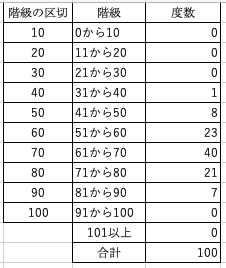
\includegraphics[width=3cm]{chap1/freq.png}
        \caption{Excelで作成した度数分布表}
        \label{fig:freq}
    \end{minipage}
    \begin{minipage}{0.5\hsize}
        \centering
        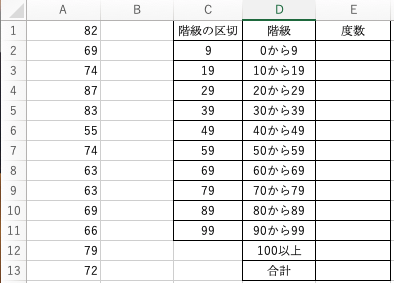
\includegraphics[width=6cm]{chap1/before_freq.png}
        \caption{Excelで作成した度数分布表}
        \label{fig:before_freq}
    \end{minipage}
\end{figure}


\begin{figure}[htbp]
    \begin{minipage}{0.5\hsize}
        \centering
        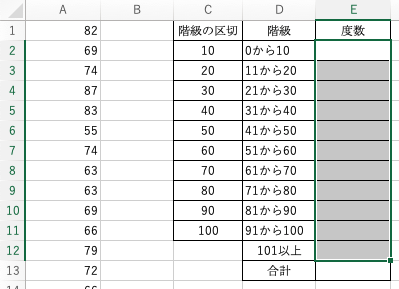
\includegraphics[width=4cm]{chap1/select_cells_freq.png}
        \caption{度数を入力するセルを選択した状態}
        \label{fig:select_cells_freq}
    \end{minipage}
    \begin{minipage}{0.5\hsize}
        \centering
        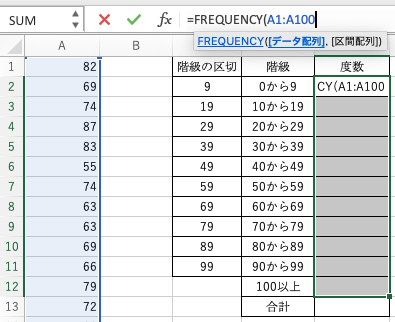
\includegraphics[width=7cm]{chap1/select_data_freq.png}
        \caption{データを選択した状態}
        \label{fig:select_data_freq}
    \end{minipage}
\end{figure}

\begin{figure}[htbp]
    \centering
    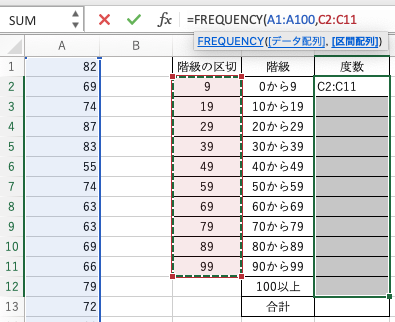
\includegraphics[width=6cm]{chap1/select_classes_freq.png}
    \caption{階級を選択した状態}
    \label{fig:select_classes_freq}
\end{figure}

\paragraph{演習}

glucoselevel.csvデータから度数分布表を書きなさい.ただし,階級は,60以下,60より大きく80以下,80より大きく100以下,100より大きく120以下,120より大きく140以下,140より大きく160以下,160より大きく180以下,180より大きい としなさい\footnote{http://www.qmss.jp/databank/medcomed/default.htmの血糖値データを用いました.}.

\subsection{ヒストグラム}

\ref{sec:hist}節で作成した度数分布表から図\ref{fig:histogram}に示すヒストグラムを作ります.
横軸は内容,縦軸は度数とします.
作る手順は次のとおりです.\footnote{ヒストグラムもかき方が多々あるので各自の好みで.}

\begin{enumerate}
    \item リボンのInsert (挿入)を選びます.そうすると,グラフや図などの挿入ボタンがたくさん出てきます.
    \item 図\ref{fig:select_cells_hist}のようにセルを選択します.
    \item リボンの挿入を押します.
    そして,リボンにある棒グラフアイコンを押し,図\ref{fig:select_barchart_hist}に示す棒グラフボタンを押します.
    そうするとヒストグラムが出来上がります.
    \item ヒストグラムの棒の幅を変えたい場合は,ヒストグラムの棒を図\ref{fig:select_bar_hist}のように選択し,図\ref{fig:select_width_hist}のGap Width (要素の間隔)を0にします.
    そうすると図\ref{fig:histogram}のようなヒストグラムが完成します.
\end{enumerate}

\begin{figure}[htbp]
    \begin{minipage}{0.5\hsize}
        \centering
  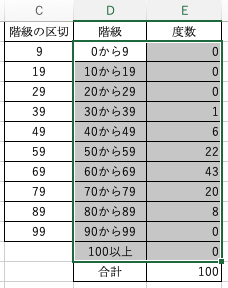
\includegraphics[width=4cm]{chap1/select_cells_hist.png}
  \caption{セルを選択した状態}
  \label{fig:select_cells_hist}
 \end{minipage}
 \begin{minipage}{0.5\hsize}
        \centering
  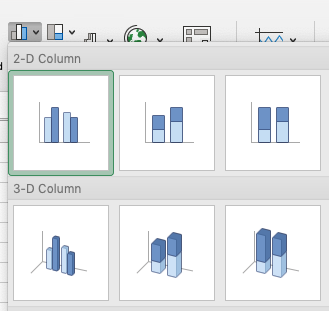
\includegraphics[width=6cm]{chap1/select_barchart_hist.png}
  \caption{棒グラフを選択する}
  \label{fig:select_barchart_hist}
 \end{minipage}
\end{figure}

\begin{figure}[htbp]
    \begin{minipage}{0.5\hsize}
        \centering
        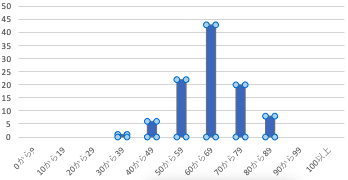
\includegraphics[width=7cm]{chap1/select_bar_hist.png}
        \caption{棒を選択した状態}
        \label{fig:select_bar_hist}
    \end{minipage}
    \begin{minipage}{0.5\hsize}
        \centering
        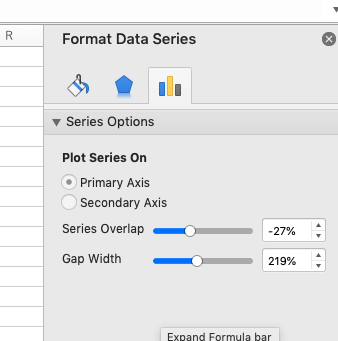
\includegraphics[width=4cm]{chap1/select_width_hist.png}
        \caption{棒の太さを選ぶ画面}
        \label{fig:select_width_hist}
    \end{minipage}
\end{figure}


\paragraph{演習}

\ref{sec:freq}節の演習で作成した度数分布表に基づきヒストグラムをかけ.

\subsection{レポート提出}

レポートテンプレートを参考にに演習の結果にまとめ,kazuhisa.fujita@komatsu-u.ac.jpへ電子データとして提出しなさい.データ形式はpdfとする.レポートの提出期限は次回の講義日までとします
